
\centering
% for double arrows a la chef
% adapt line thickness and line width, if needed
\begin{tikzpicture}[thick]
\node[] (start) {};
 \node[draw,circle,minimum size=1.5cm,left = 0.5cm of start] (f) {f$_{\text{compute}}$};
 \node[draw,right = 0.5cm of start,circle,minimum size=1.5cm] (K) {$\kse
\midtheta$};
 %\node[below left of=f_K,xshift=-1.7cm,yshift=-0.1cm] (theta) {$\bm{\theta} \sim P(\bm{\theta})$};
 \node[draw,rectangle,below=1.2cm of start, text width = 8cm] (gpmem) {\centering\texttt{gpmem}\vspace{1mm}

\small$\text{memo table} = (\xbf,\ybf)$\vspace{0.7mm}

\small$\;\;\;\;\;\;\;\;\;\;P(f_{emu}(x) \mid \xbf,\ybf,\thetabf)\sim
\mathcal{N}\big(\mupost,\Kpost)\big)$
 };
%  \node[draw,rectangle,color=ForestGreen,below = .1ex of gpmem,minimum width=1.5cm, minimum height=0.4cm,yshift=0.9cm,xshift=0.3cm] (mark) {};
  \node[draw,rectangle,dashed,right=1.6cm of K, text width = 3.4cm] (math) {\footnotesize
 $\kse\,= \sigma^2 \exp(-\frac{(x-x^\prime)^2}{2\ell^2})$\vspace{1mm}

 $\thetabf \;\;\,\,= \{\sigma,\ell \} \rightarrow$ Scope\vspace{1mm}

 $\sigma\;\;\; \sim P(\sigma)\,$\vspace{1mm}

 $\ell\;\;\;\, \sim P(\ell)\;\,$\vspace{1mm}


 };
 \node[draw,rectangle,dashed,minimum size=1cm,left= 2.2cm of f] (resources)
{
\includegraphics[width=2.8cm]{figs/resources.jpg}};

\node[draw,rectangle,below=0.8cm of gpmem,text width =7cm] (f_emu) {\centering $f_{emu}$ \vspace{1mm}

\renewcommand{\arraystretch}{0.5}
\begin{tabular}{l|l}\footnotesize
  \footnotesize$x$ & \footnotesize$f(x)$ \\ \hline
  \footnotesize $x_1$  &\footnotesize$y_1$ \\
 \footnotesize  $x_2$  & \footnotesize$y_2$ \\
 \footnotesize$\cdots$ & \footnotesize $\cdots$
 \end{tabular}
 $\;\;\;\;$
 \begin{tabular}{l}
 \small Parameters:\\
\small  Kernel lengthscale $\ell$  \\
\small Kernel scale-factor $sf$
 \end{tabular}

};


\node[below = .1ex of gpmem,inner sep = 0pt,outer sep=0pt,xshift=-0.3cm] (helper1) {};
\node[below = .1ex of gpmem,inner sep = 0pt,outer sep=0pt,xshift=0.7cm] (helper2) {};

\node[above = .1ex of f_emu,inner sep = 0pt,outer sep=0pt, xshift=0mm] (helper_emu) {};

\node[above = 0.75cm of resources,inner sep = 0pt,outer sep=0pt] (helper_resource_top) {};
\node[left = 1cm of f_emu] (x_hat) {$\xprime$} ;
\node[right = 1cm of f_emu] (GaussianHat)
{$\yprime$} ;



% 1st pass: draw arrows

\draw[thick,dashed,->] (resources) --node [pos=0.5,below] {\footnotesize resource}  node [pos=0.5,above] {\footnotesize outside} (f);
\draw[thick,dashed,->] (math) -- node [pos=0.5,above] {\footnotesize Kernel} (K);
\draw[thick,->] (K) -- (gpmem);
\draw[thick,->] (f) -- (gpmem);
\draw[thick,->] (gpmem) -- (f_emu);

\draw[thick,->,dashed] (x_hat) -- (f_emu);
\draw[thick,->,dashed] (f_emu) -- (GaussianHat);

\node[above=1 cm of start] (alabel) {(a) \gpmem: Schematic};
%%%%%%%%%%%%%%%%%%%%%%%%%%%%%%%%%%%%%%%%%%%%%%%%%%%%%%%%%%%%
%%%%%%%%%%%%  Code             %%%%%%%%%%%%%%%%%%%%%%%%%%%%%
%%%%%%%%%%%%%%%%%%%%%%%%%%%%%%%%%%%%%%%%%%%%%%%%%%%%%%%%%%%%

\node[below=-0.3cm of f_emu,xshift=-1.3cm] (b_code){
\small\begin{lstlisting}[mathescape,escapechar=\#]
define f = proc(x) {exp(-0.1*abs(x-2)) * 10 * cos(0.4*x) + 0.2};#\vspace{1mm}#
assume sf  = tag(scope="hyper-parameters", gamma(5,1));
assume l   = tag(scope="hyper-parameters", gamma(5,1));
assume kse = apply_function(make_squaredexp(sf, l))#\vspace{1mm}#;
\end{lstlisting}
};
\node[below=-0.25cm of b_code,xshift=-2.3cm] (c_code){
\small\begin{lstlisting}[mathescape,escapechar=\#]
assume (f_compute, f_emu) = gpmem(f, kse);#\vspace{1mm}#
sample f_emu(array(-20, $\cdots$, 20));
\end{lstlisting}
};

\node[below=0.2cm of c_code,xshift=-0.95cm] (d_code){
\small\begin{lstlisting}[mathescape,escapechar=\#]
predict f_compute(12.6);#\vspace{1mm}#
sample  f_emu(array(-20, $\cdots$, 20));
\end{lstlisting}
};

\node[below=0.5cm of d_code] (e_code){
\small\begin{lstlisting}[mathescape,escapechar=\#]
predict f_compute(-6.4);#\vspace{1mm}#
sample  f_emu(array(-20, $\cdots$, 20));
\end{lstlisting}
};

\node[below=-0.0cm of e_code] (f_code){

\small\begin{lstlisting}[mathescape,escapechar=\#]
observe f_emu(-3.1) =  2.60;
observe f_emu(7.8)  = -7.60;
observe f_emu(0.0)  = 10.19;#\vspace{1mm}#
sample  f_emu(array(-20, $\cdots$, 20));

\end{lstlisting}
};

\node[below=0.0cm of f_code,xshift=1.2cm] (g_code){
\small\begin{lstlisting}[mathescape,escapechar=\#]
infer mh(scope="hyper-parameters", steps=50);#\vspace{1mm}#
sample f_emu(array(-20, $\cdots$, 20));
\end{lstlisting}
};

% samples/curve images
\node[right=-4.5cm of b_code,yshift=-2.2cm] (c_pic){
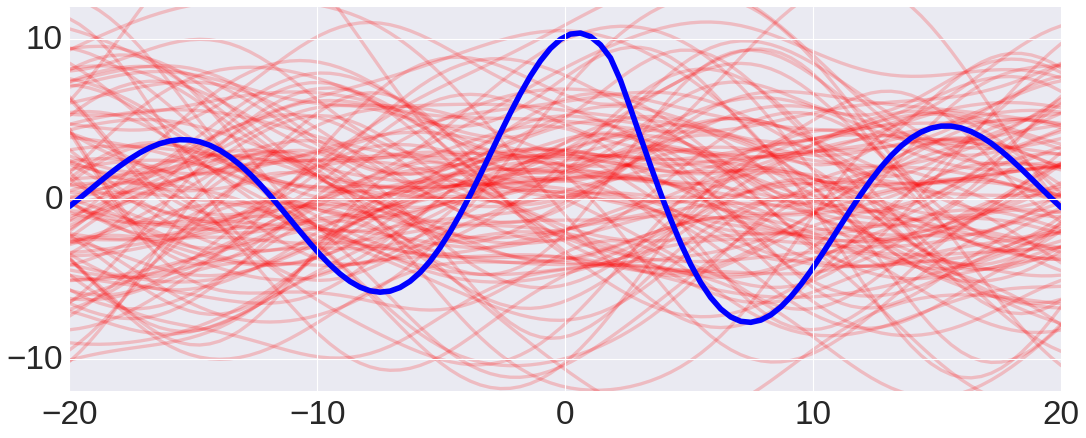
\includegraphics[height=2.0cm]{figs/tutorial_1.png}
};
\node[below=-0.1cm of c_pic] (d_pic){
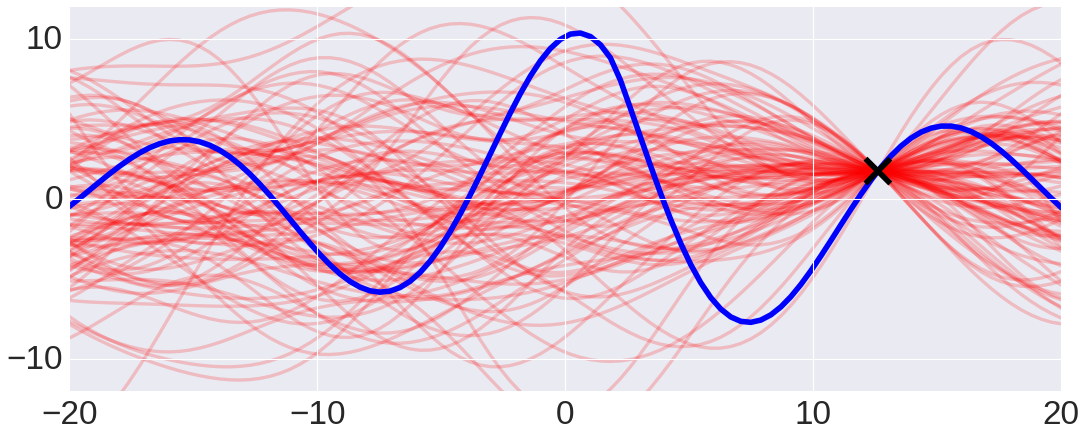
\includegraphics[height=2.0cm]{figs/tutorial_2.png}
};
\node[below=-0.1cm of d_pic] (e_pic){
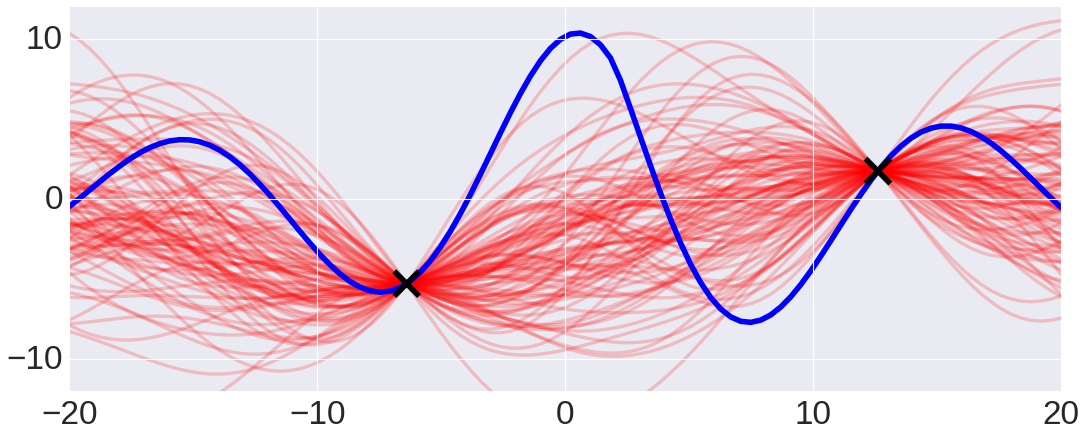
\includegraphics[height=2.0cm]{figs/tutorial_3.png}
};
\node[below=-0.1cm of e_pic] (f_pic){
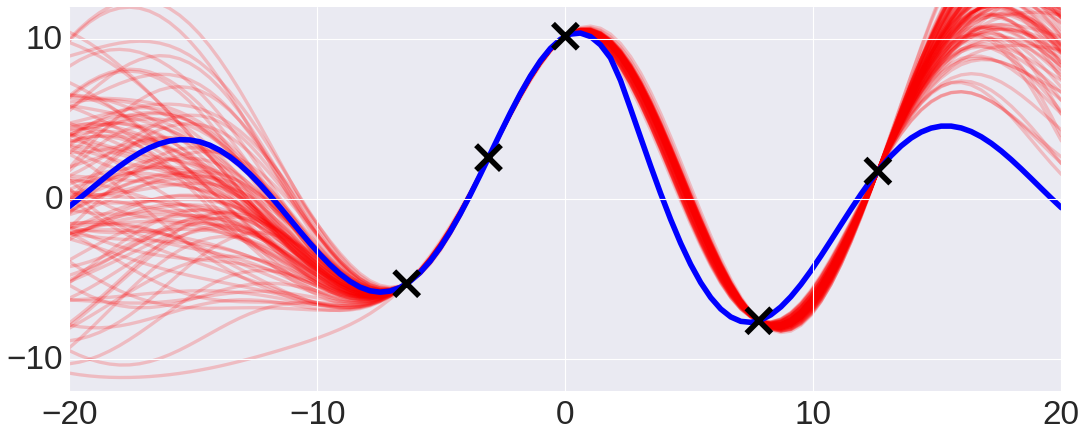
\includegraphics[height=2.0cm]{figs/tutorial_5.png}
};
\node[below=-0.1cm of f_pic] (g_pic){
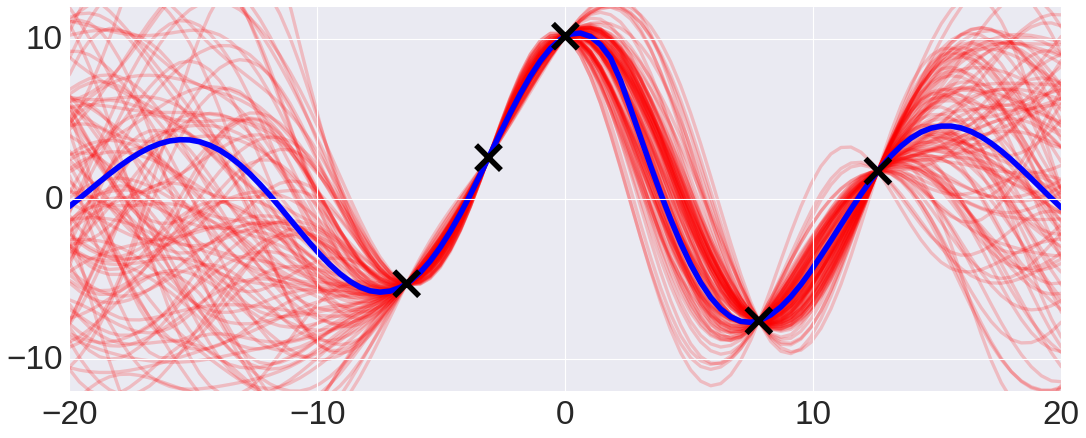
\includegraphics[height=2.0cm]{figs/tutorial_6.png}};

% horizontal lines
\draw 
  ([xshift=-0.2cm,yshift=-0.6cm]b_code.north west) --
([xshift=0.8cm,yshift=-0.6cm]b_code.north east); 
\draw 
  ([xshift=-0.2cm,yshift=0.2cm]b_code.south west) -- ([xshift=0.8cm,yshift=0.2cm]b_code.south east);   
 \draw 
  ([xshift=-0.2cm,yshift=-1.9cm]b_code.south west) -- ([xshift=0.8cm,yshift=-1.9cm]b_code.south east); 
 \draw 
  ([xshift=-0.2cm,yshift=-4.1cm]b_code.south west) -- ([xshift=0.8cm,yshift=-4.1cm]b_code.south east); 
 \draw 
  ([xshift=-0.2cm,yshift=-6.3cm]b_code.south west) -- ([xshift=0.8cm,yshift=-6.3cm]b_code.south east); 
 \draw 
  ([xshift=-0.2cm,yshift=-8.5cm]b_code.south west) -- ([xshift=0.8cm,yshift=-8.5cm]b_code.south east); 

% arrows
% (d)
\node[below = -2.45cm of d_pic,xshift=1.53cm] (arrow_d_end){};
\node[below = -1.45cm of d_pic,xshift=1.53cm] (arrow_d_head){};
\draw[green,->] (arrow_d_end) -- (arrow_d_head);
% (e)
\node[below = -1.9cm of e_pic,xshift=-0.62cm] (arrow_e_end){};
\node[below = -0.9cm of e_pic,xshift=-0.62cm] (arrow_e_head){};
\draw[green,->] (arrow_e_end) -- (arrow_e_head);
% (f)
\node[below = -2.49cm of f_pic,xshift=-0.26cm] (arrow_f_end1){};
\node[below = -1.49cm of f_pic,xshift=-0.26cm] (arrow_f_head1){};
\draw[->] (arrow_f_end1) -- (arrow_f_head1);
\node[below = -2.05cm of f_pic,xshift=0.1cm] (arrow_f_end2){};
\node[below = -1.05cm of f_pic,xshift=0.1cm] (arrow_f_head2){};
\draw[->] (arrow_f_head2) -- (arrow_f_end2);
\node[below = -2.45cm of f_pic,xshift=1.53cm] (arrow_f_end3){};
\node[below = -1.45cm of f_pic,xshift=1.53cm] (arrow_f_head3){};
\draw[->] (arrow_f_end3) -- (arrow_f_head3);

% labels
\node[below=0.9cm of f_emu,xshift=-8.5cm] (b) {(b)};
\node[below=1.4cm of b] (c) {(c)};
\node[below=1.4cm of c] (d) {(d)};
\node[below=1.4cm of d] (e) {(e)};
\node[below=1.6cm of e] (f) {(f)};
\node[below=1.5cm of f] (g) {(g)};
\end{tikzpicture}

